\documentclass[12pt,a4paper]{article}

\usepackage[utf8x]{inputenc}

%% Sets page size and margins
\usepackage[a4paper,top=2cm,bottom=2cm,left=2cm,right=2cm,marginparwidth=1.75cm]{geometry}
\usepackage[hidelinks]{hyperref}
%% Useful packages
\usepackage{amsmath}
\usepackage{hyperref}
\usepackage{graphicx}
\usepackage{array}
\usepackage{wrapfig}
\usepackage{lipsum}
\usepackage{tocloft}
\usepackage{caption}
\usepackage{listings}
\usepackage{color} %red, green, blue, yellow, cyan, magenta, black, white
\definecolor{codegreen}{rgb}{0,0.6,0}
\definecolor{codegray}{rgb}{0.5,0.5,0.5}
\definecolor{codepurple}{rgb}{0.58,0,0.82}
\definecolor{backcolour}{rgb}{0.95,0.95,0.92}

\lstdefinestyle{mystyle}{
    backgroundcolor=\color{backcolour},   
    commentstyle=\color{codegreen},
    keywordstyle=\color{magenta},
    numberstyle=\tiny\color{codegray},
    stringstyle=\color{codepurple},
    basicstyle=\footnotesize,
    breakatwhitespace=false,         
    breaklines=true,                 
    captionpos=b,                    
    keepspaces=true,                 
    numbers=left,                    
    numbersep=5pt,                  
    showspaces=false,                
    showstringspaces=false,
    showtabs=false,                  
    tabsize=2
}
\lstset{style=mystyle}

\definecolor{mygreen}{RGB}{28,172,0} % color values Red, Green, Blue
\definecolor{mylilas}{RGB}{170,55,241}
\graphicspath{{./Images}}



\begin{document}

\begin{titlepage}

    \newcommand{\HRule}{\rule{\linewidth}{0.5mm}} 							% horizontal line and its thickness
    \center

    % University
    \textsc{\LARGE University of Moratuwa}\\[1cm]

    % Document info
    \textsc{\Large FUNDAMENTALS OF IMAGE PROCESSING}\\[0.2cm]
    \textsc{\large EN2550}\\[1cm] 										% Course Code
    \HRule \\[0.8cm]
    { \Large \bfseries  INTENSITY TRANSFORMATIONS \& \\ [0.3cm]NEIGHBORHOOD FILTERING}\\[0.7cm]
    \HRule \\[2cm]
    \large
    S.Sanjith : 190562G\\[1.5cm]
    {\large \today}\\[2cm]
    
\includegraphics[width=0.4\textwidth]{mora.png}\\[1cm] 	% University logo
    \vfill
\end{titlepage}

\newpage
\tableofcontents
\vspace{12cm}
Git-hub link : \url{https://github.com/sanjith1999/EN2550-Assignments.git}
\newpage
\section{Intensity Transformation}
The first image depicts the situation where a photo of a girl is taken without a clear lighting setup. Most of the details on the right side of the face are hidden. Through stretching and increasing the brightness of such range with an intensity transformation a viewer can extract the details hidden in such range. Furthermore, through the results depicted in the image, it is obvious that with fine-tuning of brightness and contrast parameters it is possible to generate perfect photos from photos without proper lighting to an extent.
\begin{figure}[h]
    \begin{minipage}{.3\textwidth}
        \centering
        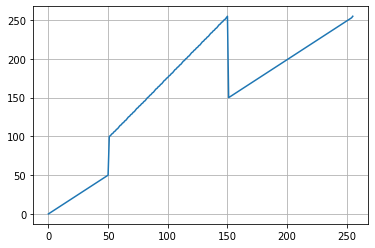
\includegraphics[width=.85\textwidth]{q1_1.png}
    \end{minipage}
    \begin{minipage}{.7\textwidth}
        \centering
        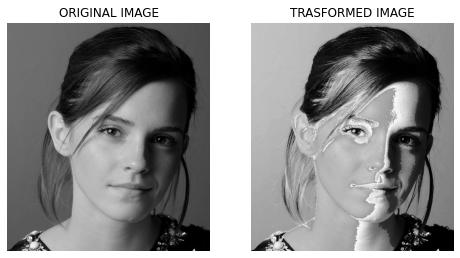
\includegraphics[width=.68\textwidth]{q1.png}
    \end{minipage}
\end{figure}


\section{Accenuation of a White \& Gray Matter }
\begin{figure}[h]
    \centering
    \begin{minipage}[c]{.6\textwidth}
        \centering
        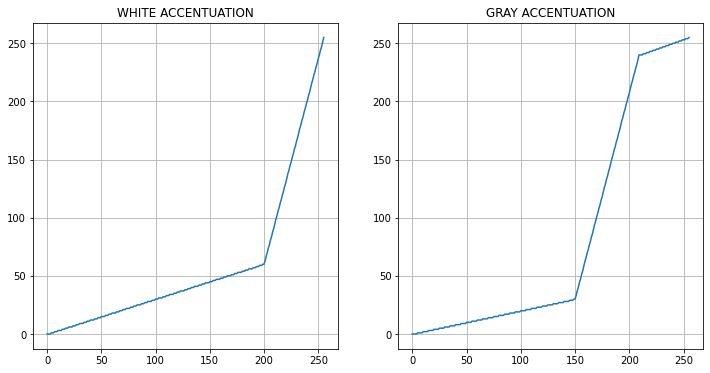
\includegraphics[width=.8\textwidth]{q2_1.png}
    \end{minipage}
    \begin{minipage}[c]{\textwidth}
        \centering
        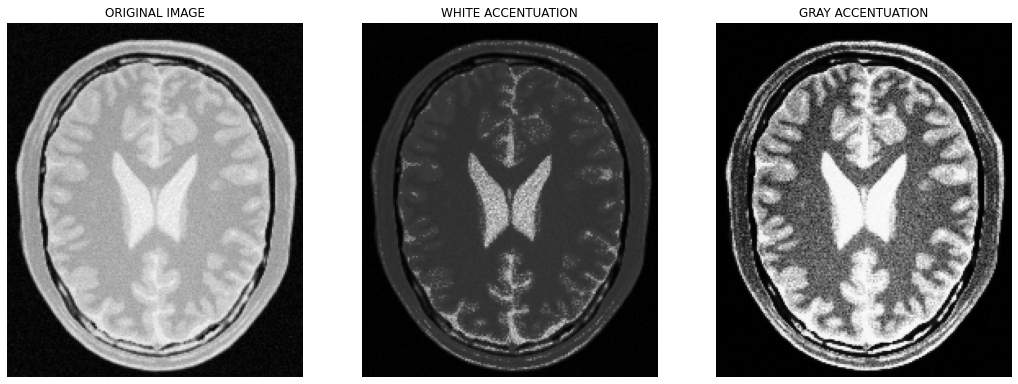
\includegraphics[width=\textwidth]{q2_2.png}
    \end{minipage}
\end{figure}
To accentuate the details in a particular intensity region we have to provide more intensity range to such a small range through intensity transformations as shown in the above plots. The above picture describes a situation where white and gray regions are being provided with a wider range of intensities to extract more information from them. The second image is the best suit for analyzing white matter and the third image for gray matter for medical diagnosing purposes.
\newpage
\section{Gamma Correction}
Gamma correction can be used to change the distribution of intensities throughout the image. In the image illustrated below, it is obvious that $\gamma>1$ will generate a darker image than the original. And $\gamma <1$ produces an image that is lighter than the original which is the best suit for this situation. So it is important to choose the best $\gamma$ according to the range of intensity distribution.
\begin{figure}[h]
    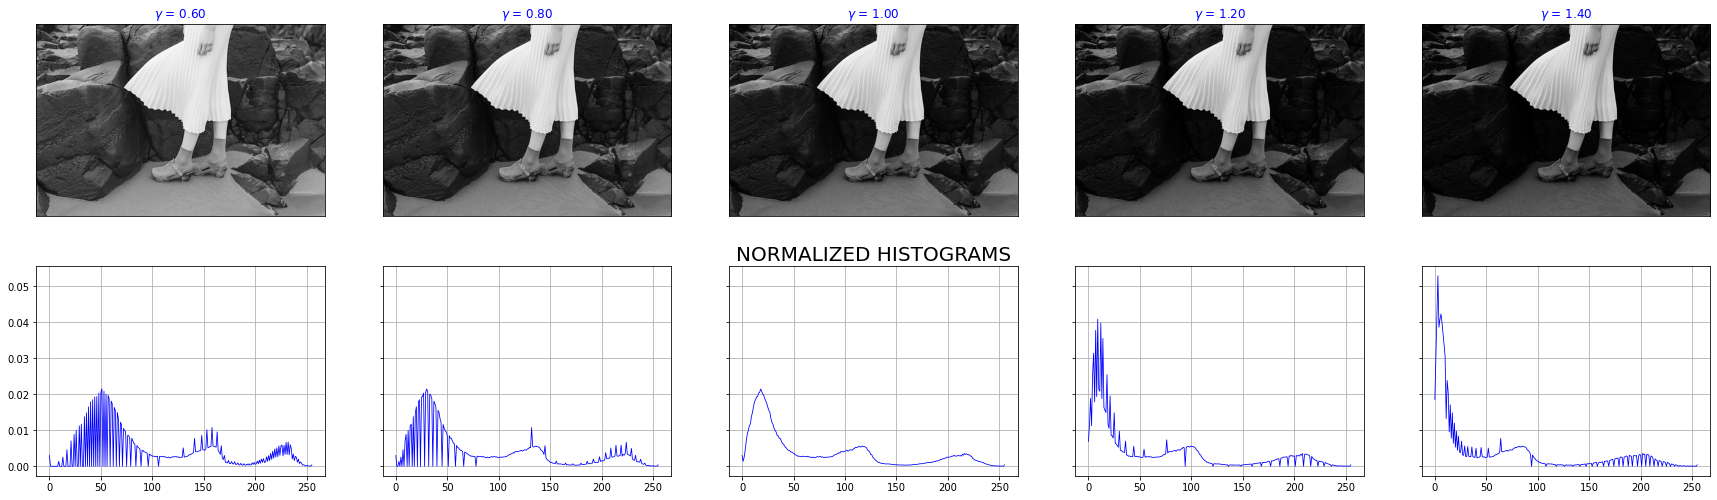
\includegraphics[width=\textwidth]{q3.png}
    \centering
\end{figure}


\section{Histogram Equalization}

\begin{figure}[h]
    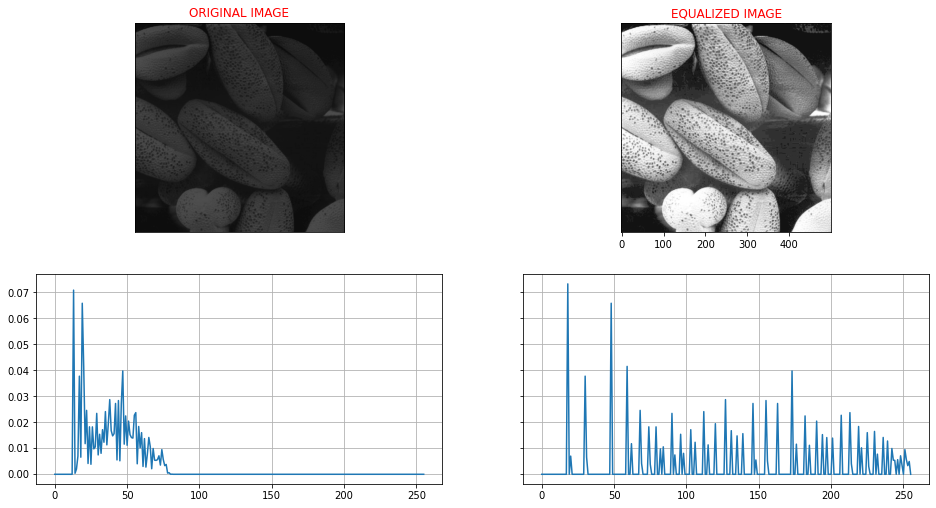
\includegraphics[width=\textwidth]{q4.png}
    \centering
\end{figure}
Histogram equalization is a technique used to equalize the distribution of intensities over the full available range. The idea is to use the normalized cumulative distribution of the original image as the intensity transformation. The above histograms depict the distribution of intensities in the original and transformed image. Although the image is darker after the transformation, intensities have been distributed all over the range. This technique is suitable for images that contain intensities contracted over a small range. The following code illustrates the implementation of this technique.
\newpage
\begin{lstlisting}
    hist_f4=cv.calcHist([f4],[0],None,[256],[0,256])
    pdf=hist_f4/np.sum(hist_f4)
    cdf=np.cumsum(pdf)
    
    t_equalization=255*cdf
    f4_equalized=cv.LUT(f4,t_equalization)
    hist_equalized=cv.calcHist([f4_equalized],[0],None,[256],[0,256])
    pdf_equalized=hist_equalized/np.sum(hist_equalized)
\end{lstlisting}

\section{Image Zoom}
Stretching the dimensions of the original image generates a larger version of the current image.
\subsection{Nearest-Neighbor Method}
Intensity approximation of a zoomed member to the nearest pixel in the original.
\begin{lstlisting}
    for row in range(zoomedImg.shape[0]):
        source_row = min(round(row/sf), img.shape[0]-1)
        for column in range(zoomedImg.shape[1]):
            source_column = min(round(column/sf), img.shape[1]-1)

            # FOR GRAY IMAGE
            if len(img.shape) == 2:
                zoomedImg[row][column] = img[source_row][source_column]
            
            # FOR COLOR IMAGE
            else:
                for channel in range(3):
                    zoomedImg[row][column][channel] = \
                        img[source_row][source_column][channel]
\end{lstlisting}


\subsection{Bi-Linear Interpolation Method}
Intensity calculation for each member of the zoomed image via linearly interpolating the four nearest neighbors in the original image.
\begin{lstlisting}
for row in range(zoomedImg.shape[0]):
    row_position = row/sf
    row_below = math.floor(row_position)
    row_up = min(math.ceil(row_position),img.shape[0]-1)
    for column in range(zoomedImg.shape[1]):
        column_position = column/sf
        column_previous = math.floor(column_position)
        column_next = min(math.ceil(column_position),img.shape[1]-1)
        delta_row = row_position - row_below
        delta_column = column_position - column_previous

        # FOR GRAY IMAGE
        if len(img.shape) == 2:  
            interVal1 = img[row_below][column_previous]*(1-delta_row)\
                + img[row_up][column_previous]*(delta_row)
            interVal2 = img[row_below][column_next]*(1-delta_row)\
                + img[row_up][column_next]*(delta_row)
            zoomedImg[row][column] = (interVal1*(1-delta_column)
                                      + interVal2*(delta_column))
\end{lstlisting}

\newpage
\subsection*{Analyzation of Results}
\begin{figure}[h]
    \centering
    \begin{minipage}[c]{\textwidth}
        \centering
        \caption*{Similarity Measure with Normalized SSD}
        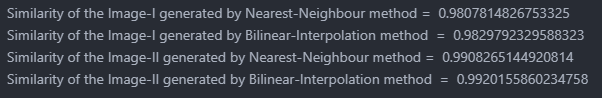
\includegraphics[width=.75\textwidth]{q5_2.png}
    \end{minipage}
    \begin{minipage}[c]{\textwidth}
        \centering
        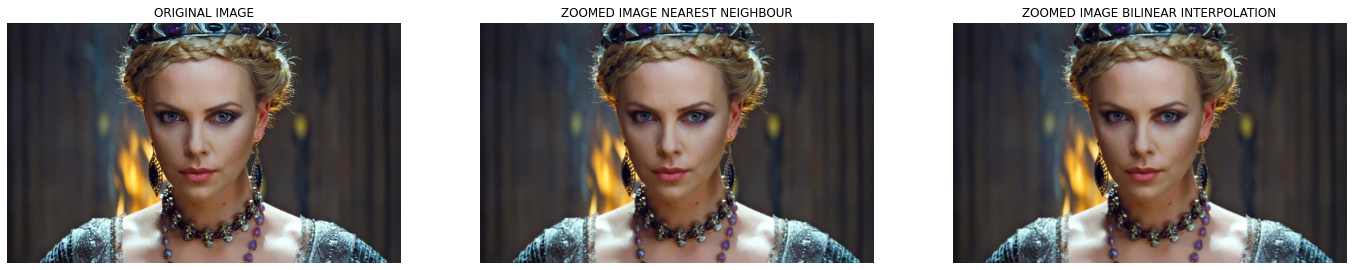
\includegraphics[width=\textwidth]{q5_1.png}
    \end{minipage}
\end{figure}
By the results obtained for similarity measure, it is obvious that bilinear interpolation yields more accurate results for zoom images. Anyhow both the methods yield the result with more than 99\% percent similarity which leads to same-looking images for human eyes. The pictures of original and zoomed images from both the methods look indistinguishable although they have similarity variation in thrid decimal point. The code used to calculate the normalized error and similarity percent is as follows.
\begin{lstlisting}
    e1_nn = cv.norm(f5_1,zoom_im1_nn, cv.NORM_L2)
    e1_bi = cv.norm(f5_1,zoom_im1_bi, cv.NORM_L2)
    similarity_nn_1 = 1 - e1_nn/(f5_1.shape[0]*f5_1.shape[1])
    similarity_bi_1 = 1 - e1_bi/(f5_1.shape[0]*f5_1.shape[1])
\end{lstlisting}
\section{Sobel Filter}
\begin{figure}[h]
    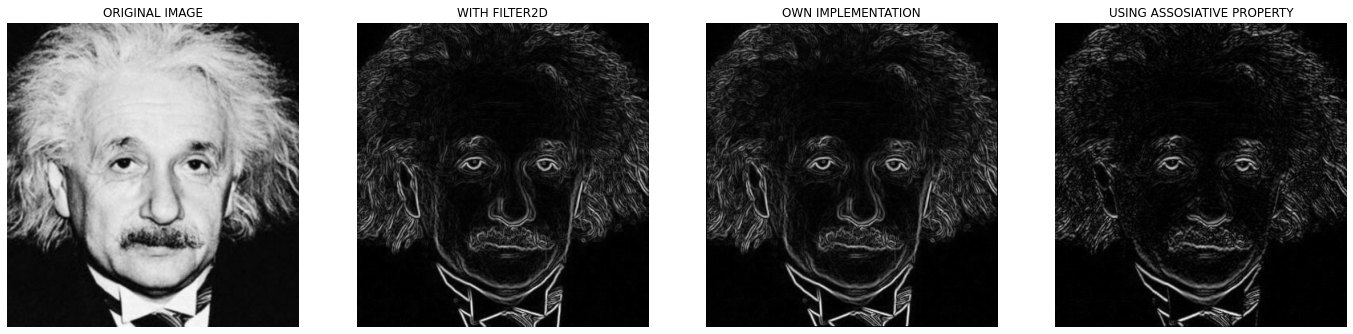
\includegraphics[width=\textwidth]{q6.png}
    \centering
\end{figure}
Sobel filter gives a good idea about the edges in an image. The images shown above are generated using a Sobel filter with different approaches. From the images, it is obvious that the filter traces out a clear edge outline of Einstein.
\par
The similarity of the results ensures the idea that convolution is associative and commutative. Although loop implementation of result yields the same result as filter2D function, it increases the computational complexity of the calculation. All the codes used to generate such images are illustrated below.
\newpage
\rule{\textwidth}{0.4pt}
\begin{lstlisting}
    kernel_v=np.array([(-1,-2,-1),(0,0,0),(1,2,1)],np.float32)
    kernel_h=np.array([(-1,0,1),(-2,0,2),(-1,0,1)],np.float32)
    
    f6_x=cv.filter2D(f6,-1,kernel_v)
    f6_y=cv.filter2D(f6,-1,kernel_h)
    f6_sobel=np.sqrt(f6_x**2+f6_y**2)
    
    # WITH OWN IMPLEMENTATION
    kernel_vo=np.array([(1,2,1),(0,0,0),(-1,-2,-1)],np.float32)
    kernel_ho=np.array([(1,0,-1),(2,0,-2),(1,0,-1)],np.float32)
    f6_xo=filter(f6,kernel_vo)
    f6_yo=filter(f6,kernel_ho)
    f6_sobel_o=np.sqrt(f6_xo**2+f6_yo**2)
    
    # USING THE ASSOSIATIVE PROPERTY
    kernel_v1 = np.array([-1, 0, 1], dtype = np.float32)
    kernel_v2 = np.array([[1], [2], [1]], dtype = np.float32)
    kernel_h1 = np.array([1, 2, 1], dtype = np.float32)
    kernel_h2 = np.array([[-1], [0], [1]], dtype = np.float32)
    
    f6_x_=cv.filter2D(f6,-1,kernel_v1)
    f6_x_=cv.filter2D(f6_x_,-1,kernel_v2)
    
    f6_y_=cv.filter2D(f6,-1,kernel_h1)
    f6_y_=cv.filter2D(f6_y_,-1,kernel_h2)
    
    
    f6_sobel_asso=(np.sqrt(f6_x_**2+f6_y_**2))
\end{lstlisting}
\rule{\textwidth}{0.4pt}

\section{Image Enhancement}
Separating foreground and background features of an image and performing filter operations appropriately, can be effectively used to enhance the images.
\par
The following sequence of images illustrates the steps of the image enhancement process. 
\par
\begin{figure}[h]
    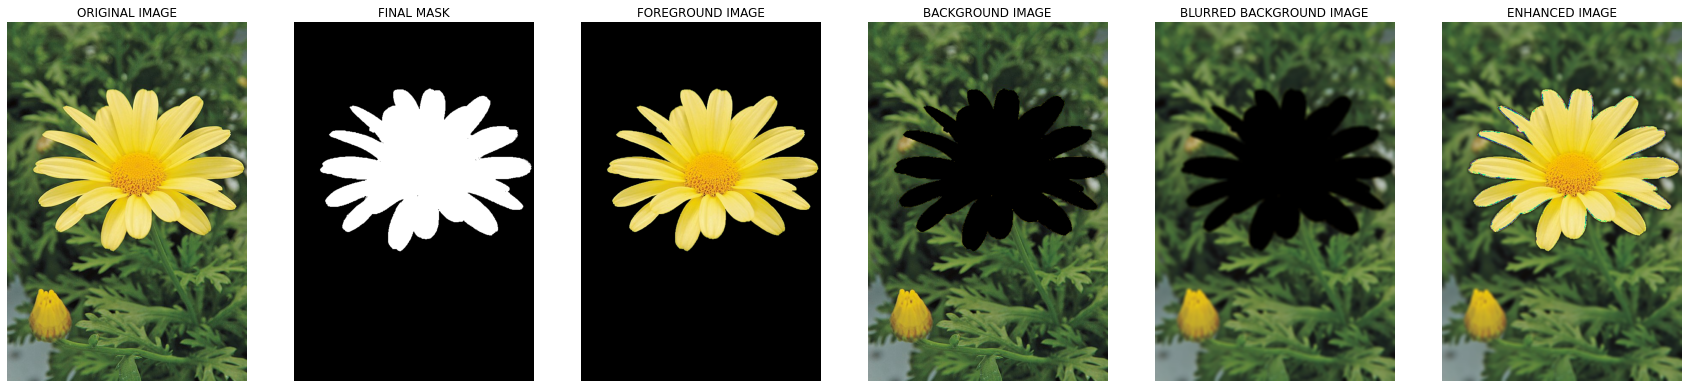
\includegraphics[width=\textwidth]{q7.png}
    \centering
\end{figure}
The background just beyond the edge of the flower is quite dark in the enhanced image. This is because when blurring the background using a gaussian kernel, the background just beyond the edge of the flower is affected by the neighboring darker pixels contained in the flower.
In the background, the flower is replaced by dark pixels.
\\
The techniques used in the image enhancement process are explained below...
\newpage
\subsection{Segmentation of Image}
By creating a loop enclosing the foreground features using the grabCut function and zeroing out all the other pixels, we can create a mask to separate the foreground image from the original image.
\begin{lstlisting}
    mask = np.zeros(f7.shape[:2],np.uint8)
    bgdModel = np.zeros((1,65),np.float64)
    fgdModel = np.zeros((1,65),np.float64)
    rect = (30,70,650,550)
    
    cv.grabCut(f7,mask,rect,bgdModel,fgdModel,5,cv.GC_INIT_WITH_RECT)
    mask2 = np.where((mask==2)|(mask==0),0,1).astype('uint8')
    fore = f7*mask2[:,:,np.newaxis]
    back = f7 - fore
\end{lstlisting}
\subsection{Blurring Background}
After separating the background pixels of an image and applying a simple Gaussian filter we can blur the background portion of the image. 
\begin{lstlisting}
    blurred_bg = cv.GaussianBlur(back, (9,9), 4)
    enhanced = fore + blurred_bg
\end{lstlisting}
\vspace{5cm}
\section*{References}
\begin{enumerate}
    \item \href{https://github.com/bimalka98/Computer-Vision-and-Image-Processing}{Similar Image Processing Project}
    \item \href{https://opencv.org/}{Opencv Home}
    \item \href{https://www.tutorialspoint.com/dip/sobel_operator.htm}{An Article on Usage of Sobel Operator}
    \item \href{https://medium.com/mlearning-ai/image-zoom-using-computer-vision-using-opencv-and-python-1eeaee53eeb8}{An Article on Image zooming}
    \item \href{https://pyimagesearch.com/2020/07/27/opencv-grabcut-foreground-segmentation-and-extraction/}{Tutorial on Foreground Segmentation and Extraction}
\end{enumerate}
\end{document}